\section[\thesection \  Applikation]{Applikation}\label{sec:application}

\begin{frame}{Test Inferenz auf eigene Bilder} 
        
    \begin{columns}
        \column{0.5\columnwidth}
        \begin{figure}
            \centering
            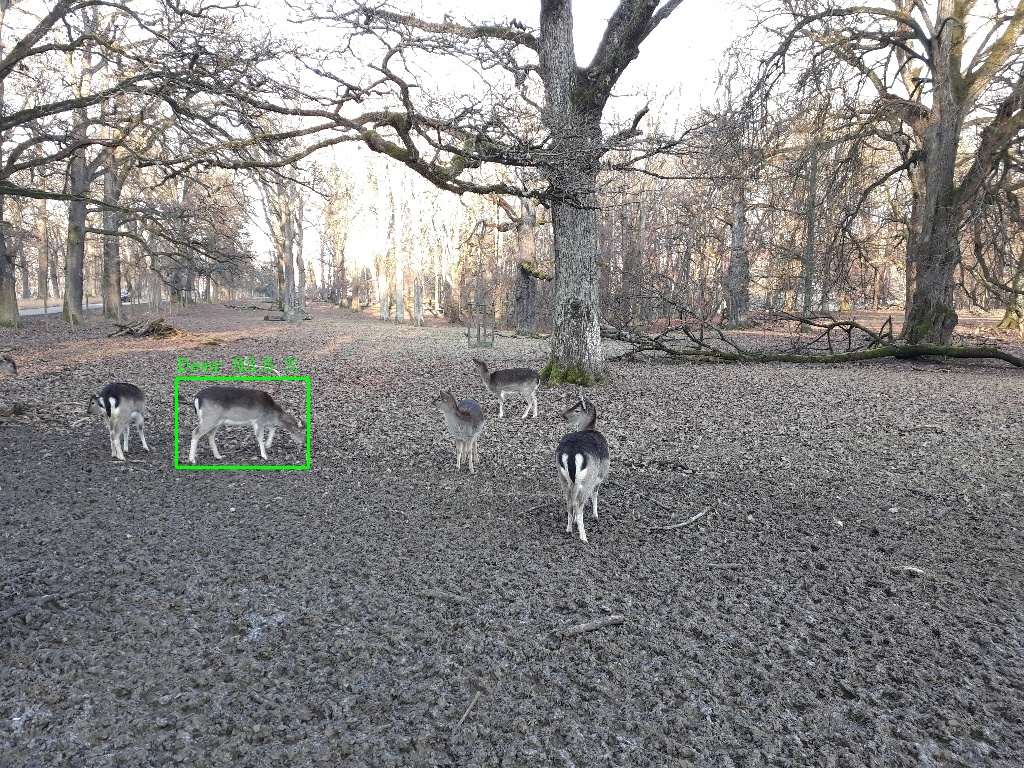
\includegraphics[width=\textwidth]{Bilder/infer_result_ssd.jpg}
            \caption{SSD+InceptionV2}
        \end{figure}
        
        \column{0.5\columnwidth}
        \begin{figure}
            \centering
            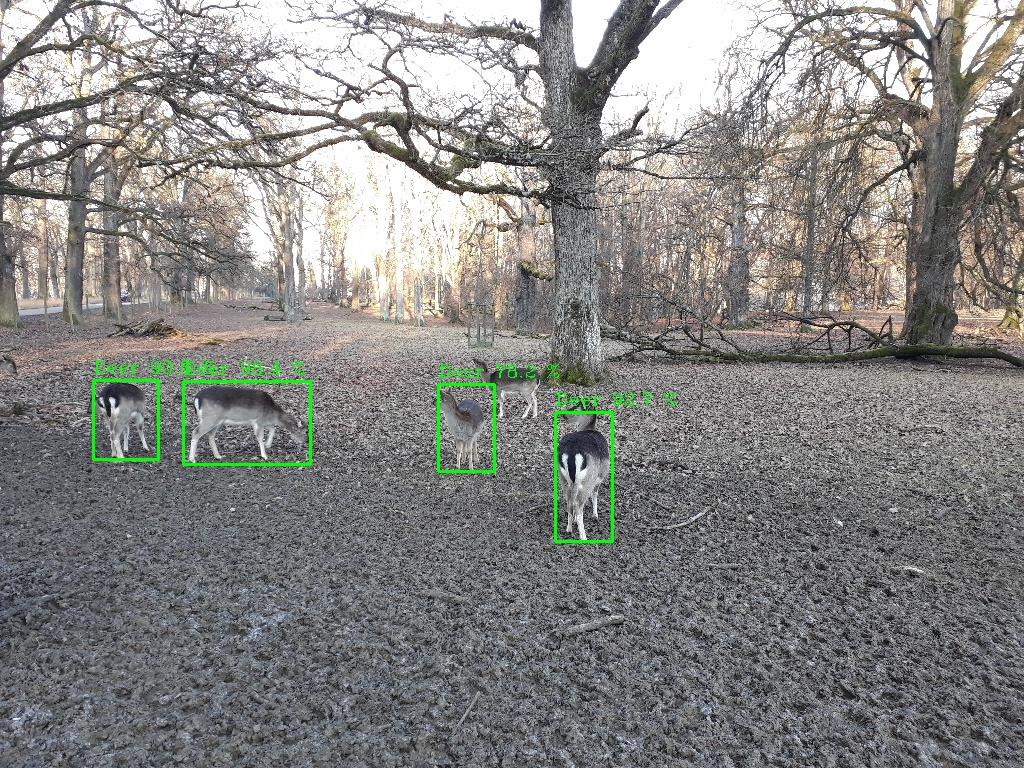
\includegraphics[width=\textwidth]{Bilder/infer_result_faster.jpg}
            \caption{Faster R-CNN+InceptionV2}
        \end{figure}
    \end{columns}

\end{frame}

\begin{frame}{Applikation}

    % Define block styles
\tikzstyle{decision} = [diamond, draw, fill=blue!20, 
    text width=3.5em, text badly centered, inner sep=0pt, text height=0.4em, node distance=2cm]
\tikzstyle{block} = [rectangle, draw, fill=blue!20, 
    text width=3em, text centered, minimum height=2em, node distance=2cm]
\tikzstyle{line} = [draw, -latex']
\tikzstyle{cloud} = [draw, ellipse,fill=red!20, node distance=2.5cm,
    minimum height=2em]
    
\begin{tikzpicture}[node distance = 2.2cm, auto]
    % place notes
    \node [cloud] (frame) {Frame};
    \node [decision, right of=frame] (motion) {Bewe-\\gung};
    \node [block, right of=motion] (buffer) {Buffer};
    \node [block, right of=buffer] (infer) {Infer};
    \node [decision, right of=infer] (thresshold) {Pred.\\> 0.8};
    \node [cloud, right of=thresshold] (server) {Server};
    
    % draw connections
    \path [line] (frame) -- (motion);
    \path [line] (motion) -- node {ja} (buffer);
    \path [line] (buffer) -- (infer);
    \path [line] (infer) -- (thresshold);
    \path [line] (thresshold) -- node {send} (server);

\end{tikzpicture}

    \visible<2->{
    
    \begin{block}{Asynchrone Inferenz}
        \begin{columns}[T]
            \column{0.3\columnwidth}
            \vspace{1cm}
            \begin{itemize}
                %\item Asynchrone Inferenzrequests auf17 mehreren Threads
                \item Inferenz läuft asynchron
            \end{itemize}
            \begin{itemize}
                \item Parallele Inferenz-Requests
            \end{itemize}
            \column{0.7\columnwidth}
            \begin{figure}[h]
                \centering
                \def\svgwidth{\columnwidth}
                \input{Bilder/synch_asynch.pdf_tex}
            \end{figure}    
        \end{columns}
    \end{block}
    }
    
\end{frame}
